\documentclass[10pt,letterpaper]{article}
\usepackage[margin=0.9in]{geometry}
\usepackage{newtxtext,newtxmath}
\usepackage{booktabs}
\usepackage{graphicx}
\usepackage[hidelinks]{hyperref}
\usepackage{caption}
\captionsetup{font=small,labelfont=bf}
\setlength{\parskip}{3pt}
\setlength{\parindent}{0pt}
\newcommand{\ms}{\,ms}
\title{Supplementary Material\\\large Repair Without Stopping: A Runtime for Online Evolution of Hybrid Code--VLA Robot Programs}
\date{}
\begin{document}
\maketitle
\vspace{-2.5em}

\section*{S0. Architecture}
\begin{figure}[h]
\centering
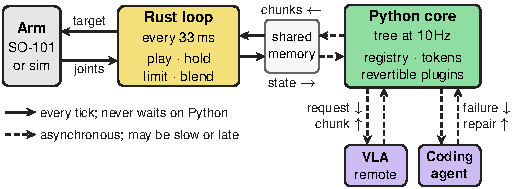
\includegraphics[width=0.6\textwidth]{fig_arch.pdf}
\caption{Runtime architecture. In our tests the arm is simulated and the VLA is a scripted placeholder.}
\end{figure}
Details omitted from the paper: if a new chunk starts more than 3\,mm from where the old one was, the jump is smoothed over five ticks (never for the gripper). Python and Rust exchange data through sequence-locked shared memory that Rust reads without waiting. Each VLA chunk carries the tick of the camera frame it used, so stale actions are skipped, as in real-time chunking (Black, Galliker and Levine 2025). Changes a plugin makes without an undo are detected but not reversed. The tree looks up each skill by name, so a repair never restarts the tree.

\section*{S1. Setup}
\textbf{System.} A Rust process ticks every 33\ms, reads a command slot and writes a state slot in shared memory (sequence-locked, one writer each), plays tick-stamped chunks of up to 50 actions, holds when no step is due, rejects chunks with non-finite values, limits speed (0.25\,m/s) and acceleration (3\,m/s$^2$), blends position gaps above 3\,mm over five ticks, and drives a kinematic hand, cube and bowl (grasp within 1.5\,cm, place within 2\,cm). Rust owns the halt record: Python writes a halt request (a counter and the highest token to halt); Rust raises its halt floor, drops every queued or playing chunk whose token is at or below it, rejects later chunks with such tokens, holds, and confirms the request in the state slot. If the Python heartbeat counter stops changing for 6 ticks (200\ms), Rust plays at most 10 more actions, then holds. A Python process runs a 10\,Hz behavior tree of plugin nodes on one asyncio loop, a bridge thread that talks to shared memory every 33\ms\ (woken at once by a halt), and worker threads for slow calls. The runtime, not the plugin, issues a halt when a node is halted, raises, or runs longer than 0.5\,s in one call (a watchdog in the bridge thread counts its own cycles, so a GIL stall cannot trigger it, and raises an exception inside the stuck call). Plugins load as generators that yield one undo per effect. A repair is kept if the next 3 episodes that \emph{start} after it goes live succeed. The stand-in VLA waits a set delay, then returns a 50-step chunk that descends 5\,cm and closes the gripper; its first steps hold the current pose to cover the expected delay.

\textbf{Machines.} \emph{A}: cloud VM, 2 vCPU (Xeon, 2.1\,GHz), 7.8\,GB; Rust pinned to core 0 with \texttt{SCHED\_FIFO} priority 50, Python pinned to core 1. \emph{B}: a laptop (Intel i7-10610U) running a 2-vCPU, 3\,GB Linux VM; Rust at \emph{normal} priority and not pinned (no real-time permission, so the launcher falls back to a plain start), Python pinned to core 1. Neither machine has a GPU.

\textbf{Metrics.} \emph{Late tick}: the command reached the driver more than 33\ms\ after its scheduled time (Rust's own clock). \emph{Command gap}: time between two consecutive driver writes. \emph{Python silence}: longest gap between the bridge thread's writes. \emph{State unchanged}: hash of blackboard, settings and ownership record equal just before and just after the registry switch (it shows the switch touches no task state; a restart discards it). \emph{Identical runtime}: same live-version map, registry size, loaded plugins, plugin modules, thread count, task count and settings hash before a bad repair and after its rejection or rollback. \emph{Idle point}: the node is not running, none of its chunks is queued or playing, and no VLA call is in flight.

\textbf{Versions.} All results below use the final code, except S9 (real SmolVLA timing), the Python-only-halt baseline in S5, the stall baselines, and B's Rust-alone run, which were measured with the earlier version (Python-side halts only; the Rust loop's timing path is the same).

\section*{S2. Control during Python stalls}
Each condition: A $3\times60$\,s, B $2\times60$\,s of pick-and-place. Baselines (unchanged code, measured earlier) run under the same stalls: A $3\times60$\,s on Rust's core and priority, B $1\times30$\,s. \emph{sync}: a loop that calls the VLA inline; \emph{threaded}: a 33\ms\ control thread with VLA calls in a worker thread. The synchronous loop is modeled as stopping at the first plugin error (no exception handling).

\begin{table}[h]
\centering\small
\begin{tabular}{lrrrrrr}
\toprule
& \multicolumn{4}{c}{Ours} & \multicolumn{2}{c}{Baselines: worst gap}\\
\cmidrule(lr){2-5}\cmidrule(lr){6-7}
Condition & ticks & late & max gap & Py silent & threaded & sync\\
\midrule
\multicolumn{7}{l}{\emph{Machine A (cloud VM, real-time priority)}}\\
VLA 0.3\,s & 5727 & 0 & 62 & 47 & 87 & 334\\
VLA 1\,s & 5727 & 2 & 75 & 99 & 88 & 1051\\
VLA 2\,s & 5727 & 1 & 84 & 66 & 69 & 2038\\
GIL-holding call & 5727 & 0 & 43 & 1686 & 1411 & 1406\\
plugin throws & 5727 & 15 & 165 & 142 & 81 & stops\\
Python killed & 5727 & 2 & 94 & -- & -- & --\\
\midrule
\multicolumn{7}{l}{\emph{Machine B (laptop VM, normal priority)}}\\
VLA 0.3\,s & 3818 & 0 & 33 & 34 & 33 & 334\\
VLA 1\,s & 3818 & 0 & 33 & 34 & 33 & 1034\\
VLA 2\,s & 3818 & 0 & 35 & 34 & 33 & 2035\\
GIL-holding call & 3818 & 0 & 34 & 2671 & 2278 & 2246\\
plugin throws & 3818 & 0 & 34 & 34 & 33 & stops\\
Python killed & 3818 & 0 & 33 & -- & -- & --\\
\bottomrule
\end{tabular}
\caption{Rust command stream while Python is stalled (gaps in ms). Rust alone: A 0 of 9{,}090 ticks late (worst gap 65\ms); B 0 of 4{,}848 (38\ms). On A, 14 of the 15 late ticks under ``plugin throws'' fell in one 0.66\,s burst in one run; its cause is unknown (B, same code, had none).}
\end{table}

\begin{figure}[h]
\centering
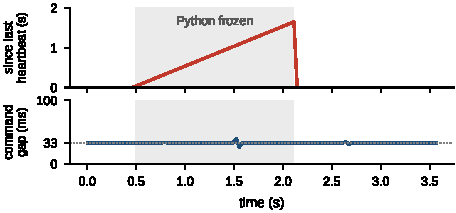
\includegraphics[width=0.55\textwidth]{fig_gil.pdf}
\caption{Machine A, GIL-holding call: Python is frozen (top: time since Rust last saw a heartbeat) while Rust keeps commanding every 33\ms\ (bottom).}
\end{figure}

Task success is not the point of this test. At 0.3\,s all episodes succeeded (A 30/30, B 20/20); at 1\,s and more the stand-in's 50-step chunk (1.65\,s) cannot cover delay plus grasp, so grasps time out while the arm holds.

\section*{S3. Live repair versus restart}
Every run starts with approach v1 (3\,cm aim error); after two failed episodes the repair is ready at an episode boundary. Swap: load beside v1, go live at the idle point, keep only if the next 3 episodes succeed. Restart: kill the Python process and start it with the fix (Rust keeps running and holds). 10 runs per condition and machine.

\begin{table}[h]
\centering\small
\begin{tabular}{llrrrrl}
\toprule
Machine & Condition & late & max gap & fix live & later ok & outcome\\
\midrule
A & swap (ours) & 0 & 65 & 198 & 30/30 & kept 10/10, state unchanged 10/10\\
 & restart & 12 & 279 & 264 & 30/30 & restarted\\
 & crashing fix, swap & 1 & 70 & -- & -- & failed, identical 10/10\\
 & crashing fix, restart & 0 & 33 & -- & -- & no runtime 10/10\\
 & failing fix, swap & 1 & 81 & 198 & 0/30 & rolled back, identical 10/10\\
\midrule
B & swap (ours) & 0 & 40 & 198 & 30/30 & kept 10/10, state unchanged 10/10\\
 & restart & 0 & 33 & 528 & 30/30 & restarted\\
 & crashing fix, swap & 0 & 34 & -- & -- & failed, identical 10/10\\
 & crashing fix, restart & 0 & 33 & -- & -- & no runtime 10/10\\
 & failing fix, swap & 0 & 34 & 198 & 0/30 & rolled back, identical 10/10\\
\bottomrule
\end{tabular}
\caption{Late ticks summed over runs; ``later ok'' for a swap counts its 3 trial episodes; gaps and ``fix live'' (median time from repair ready to the fix's first chunk on the arm, including a 150\ms\ scene reset) in ms. After a rollback, v1 (still buggy) keeps driving, so later episodes fail. All 12 late ticks of A's restarts came from one run (worst gap 279\ms). Earlier leak check: 100 load/unload plus 100 crashed-load cycles returned registry, plugin and module counts to their start.}
\end{table}

\textbf{Restart with the real VLA's weights.} Same protocol on A, but the Python process loads the real SmolVLA (450M parameters) at start, as a deployed runtime would; grasps still use the stand-in chunk so episodes can succeed on CPU. A restart must load the model again; a swap never touches it. Fix live: swap 198\ms\ in 10/10 runs (kept 10/10); restart 19.7--22.7\,s (median 20.2\,s), during which Rust held the arm. Late ticks: 2 in each condition (worst gap 83\ms). Weights were in the page cache; a cold start would be slower.

\section*{S4. Repair requested in the middle of a skill}
As the swap above, but the fix becomes ready 50\ms\ after approach v1 starts driving the arm, so the swap must wait for approach's idle point. A ($n{=}10$): wait 413--514\ms, kept 10/10, state unchanged 10/10, no ownership mismatch at the switch, hand step never above the speed cap (max 8.16\,mm per tick vs 8.25), 30/30 later episodes succeeded, 2 late ticks. B ($n{=}10$): wait 504--612\ms, kept 10/10, 0 late ticks, 30/30.

\section*{S5. Halting chunks that are already in Rust}
A code node's chunk is in Rust, either queued (start 10 ticks ahead) or playing (halt 0.35\,s into it). The node is halted and a new owner takes over at once, but the new owner's chunk arrives only later (0.6\,s for the queued case, as a VLA call would). Python polls the state slot for Rust's confirmation.

\begin{table}[h]
\centering\small
\begin{tabular}{llrrrrr}
\toprule
Machine & Case & trials & confirm median & confirm max & halted steps after request & new chunk played\\
\midrule
A & queued & 50 & 1.3\ms & 33.3\ms & 0 & 50/50\\
A & playing & 50 & 19.1\ms & 19.5\ms & 0 & 50/50\\
B & queued & 40 & 32.8\ms & 33.1\ms & 0 & 40/40\\
B & playing & 40 & 18.0\ms & 18.4\ms & 0 & 40/40\\
\bottomrule
\end{tabular}
\caption{Rust-owned halts. Confirmation times depend on where in the 33\ms\ tick the request lands; all fall within one tick.}
\end{table}

\textbf{Baseline: halting in Python only.} With the earlier version, where only Python knew a token was halted, the queued chunk played in every trial (A 50/50, B 45/45; up to 14 steps, 0.46\,s) until the new owner's chunk arrived.

\section*{S6. Stale actions}
Machine A 50 trials per case, machine B 40; all passed on both. (a) A reply carrying a cancelled token never played, including when forced into the inbox so that only the bridge's send-time check could stop it. (b) A halt with a queued chunk: it played 0 steps; with a playing chunk: it stopped mid-chunk and the arm held from the next tick. (c) Every played step (563 on A, 463 on B) matched a chunk Python sent, with a valid token and step index $=$ tick $-$ start.

\section*{S7. Faulty repairs (machine A)}
Each trial: the robot runs a working approach for one episode; a faulty repair of approach is loaded and tried (trial $k{=}3$); three more episodes follow. Rust's log is the judge. \emph{Plain reload} is the usual hot reload: import the file, run its setup, make it live at once; no undo log, trial or rollback. It still runs on our Rust loop, with Rust-owned halts and the watchdog.

\begin{table}[h]
\centering\small
\begin{tabular}{lllrl}
\toprule
Faulty repair & What it does & Ours (10 runs each) & later ok & Plain reload (5 each)\\
\midrule
raises during load & registers, then raises & rejected, identical & 30/30 & registration left behind\\
syntax error & does not parse & rejected, identical & 30/30 & stray module left\\
raises after sending & raises once its chunk is in Rust & chunk halted, rolled back & 30/30 & live; 0/15 later ok\\
endless loop & loops forever after sending & watchdog (20 fires), rolled back & 30/30 & live; 0/15\\
NaN actions & chunk with NaN positions & Rust rejected 10/10, rolled back & 30/30 & live; 0/15\\
forged token & stamps a token it does not own & never sent, rolled back & 30/30 & live; 0/15\\
aims 1\,m away & target outside workspace & limits held, rolled back & 30/30 & live; 0/15\\
wrong aim, leaks thread & starts a thread, no undo & rolled back; thread left & 30/30 & live; 0/15\\
blocks 0.3\,s per tick & correct but slow & kept & 30/30 & live; 15/15\\
crashing halt() & correct, halt() raises & halts still applied, kept & 30/30 & live; 15/15\\
\bottomrule
\end{tabular}
\caption{Over all 100 trials of ours: 22 of 104{,}270 ticks late (worst gap 163\ms), every commanded pose finite and inside the workspace, hand step never above the 8.25\,mm cap, and 0 steps played from a halted token. ``Identical'' holds for all rejected and rolled-back repairs except the thread leak, whose extra thread is detected by the fingerprint but not removed. Plain reload: 11 of 49{,}678 ticks late.}
\end{table}

\textbf{The NaN check.} Given the same NaN positions, the earlier Rust loop happened to hold (NaN comparisons zeroed the velocity), but a NaN gripper value passed straight through to the gripper command; the check now rejects the whole chunk.

\section*{S8. Agent-written repairs (machine A)}
We planted five bugs in approach, one per file, written plainly (no hint comments): the aim is 3\,cm off in $x$; the hand-off height is fixed at 12\,cm instead of the setting (5\,cm); $x$ and $y$ are swapped; the sign of $y$ is flipped; the node declares success when within 3\,cm of its target, while still moving. Each session starts the robot with one bug. Once two episodes have failed, DeepSeek-V4.1-Flash (\texttt{deepseek-flash}, called in a worker thread, so the tree and the arm never wait for it) receives: a system prompt (repair one plugin while the robot runs; reply with the whole file); a description of the plugin API and of the approach node's job (bring the open gripper to the hand-off point; the VLA then descends 5\,cm and closes; a grasp needs the gripper within 1.5\,cm of the cube centre); the current plugin source; and a failure report made only of what the robot observes (hand pose where approach ended, the seen cube pose, the hand and cube poses when the gripper closed, grasped or not, and any errors). The reply's code is loaded as a Cordis swap with a 3-episode trial. A rejected or rolled-back reply would be reported back with the load error or the trial's report, up to 3 attempts. Five sessions per bug.

\begin{table}[h]
\centering\small
\begin{tabular}{lrrrrr}
\toprule
Bug & sessions & kept at 1st reply & reply (s) & report to fix kept (s) & late ticks\\
\midrule
aim 3\,cm off & 5 & 5 & 4.0--13.0 & 21.7--37.1 & 0\\
wrong height & 5 & 5 & 5.6--16.3 & 25.5--41.4 & 1\\
$x$/$y$ swapped & 5 & 5 & 2.3--9.2 & 21.6--33.5 & 0\\
$y$ sign flipped & 5 & 5 & 5.8--10.1 & 25.7--33.6 & 1\\
stops 3\,cm early & 5 & 5 & 10.5--41.0 & 32.7--65.5 & 1\\
\bottomrule
\end{tabular}
\caption{Agent-written repairs. ``Report to fix kept'' includes the agent's reply, the wait for the idle point and the 3-episode trial. Over all sessions 3 of 45{,}038 ticks were late (worst gap 68\ms), and the three episodes after each kept fix succeeded (75/75).}
\end{table}

\begin{figure}[h]
\centering
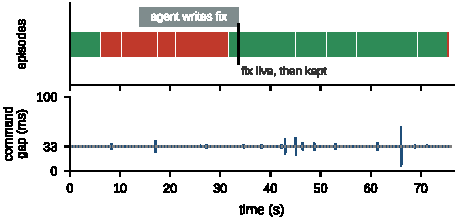
\includegraphics[width=0.6\textwidth]{fig_agent.pdf}
\caption{One session (``stops 3\,cm early''). Episodes fail while the agent writes its fix; the fix goes live at the idle point, passes its trial and is kept; the Rust command gap stays at 33\ms\ throughout.}
\end{figure}

Every reply was correct at the first attempt, so these sessions exercise the loop, not rollback of agent code; faulty code is covered in S7. Prompts, replies and failure reports for every session are included with the code.

\section*{S9. The real SmolVLA on the same CPU}
We loaded the real SmolVLA (\texttt{lerobot/smolvla\_base}, 450M parameters, 50-step chunks, 10 flow steps) on machine A's CPU and called it at every grasp; its six-joint output does not drive the Cartesian toy sim, so this measures inference time and CPU contention only. One chunk took a median 2.7\,s with two PyTorch threads (shared set-up) and 3.5--3.6\,s with one (isolated): longer than the 1.65\,s a 50-step chunk lasts at 30\,Hz, so on CPU the arm must hold between chunks and grasps fail. \emph{Isolated} (Rust real-time on core 0; Python and PyTorch with one thread on core 1), $3\times60$\,s: 0 of 7{,}109 ticks late, 99th-percentile lateness 0.33--0.48\ms. \emph{Shared} (no pinning, normal priority, two PyTorch threads): 2 of 6{,}938 late, 99th-percentile lateness 3.1--3.9\ms\ (6--12$\times$ higher), worst gap 106\ms. PyTorch releases Python's lock during inference, so the tree and bridge stayed responsive in both.

\section*{S10. Physics simulation (MuJoCo SO-101)}
The simulator runs at 500\,Hz (2\,ms step) in its own process with the MuJoCo Menagerie SO-101 model; the cube is held by friction alone. An inverse-kinematics adapter turns the Cartesian chunks into joint targets, with the wrist roll set from the cube's yaw. With the correct skill, 20/20 pick-and-place episodes succeeded. In the 60\,s demo run (Figure 1 of the main paper): v1 failed 2/2 episodes; the fix went live 3\,ms after it arrived and was kept after 3/3 trial episodes; the NaN repair was rejected by Rust (0 steps played) and rolled back in 0.2\,s; v3 was halted by the safety check at 29.6\,mm, came no closer than 18.6\,mm, with 0\,N contact, and was rolled back in 0.36\,s; 8/8 episodes after the fix succeeded. Tick lateness: max 8.7\,ms, 99th percentile 0.31\,ms. The fix and faulty repairs arrived between episodes.

\textbf{Halt test.} The arm was driven straight at the bowl, 10 runs per condition. Rust halt at 3\,cm: 0/10 contacts, stopped within 114--144\,ms, clearance 13--19\,mm. No halt: 10/10 contacts. Halt in Python only: 10/10 contacts (24--33\,N), because chunks already in Rust kept playing.

\section*{S11. Long run: an LLM agent plans, writes and repairs its own program, with a real VLA}
\textbf{Setup.} The LIBERO-Goal kitchen (MuJoCo, Franka arm) runs as the plant; our Rust loop ticks at 4\,Hz (not 30\,Hz, because LIBERO physics is slow on this CPU) and the simulator takes one LIBERO control step per tick (about 0.25$\times$ real time on this 2-core CPU). The VLA is the real SmolVLA fine-tuned on LIBERO (\texttt{HuggingFaceVLA/smolvla\_libero}, no training by us), running on the same CPU in a worker thread (median 3.2\,s per inference; the arm holds while it thinks). DeepSeek-V4.1-Flash gets one goal (``the black bowl on the stove with the stove turned on, and the wine bottle on the wine rack''), a short plugin API (behavior-tree nodes; a VLA skill that takes an English instruction; a straight-line move skill; gripper; checks), and what the robot perceives (object positions and symbolic facts). It plans the task, writes the program as plugins, and receives a report after each run. The runtime loads each batch of files live, switches it in at an idle point, and keeps it only if the task checker sees progress and nothing misbehaved (unlike the 3-episode trial of the other sections, since this job is not repeated); otherwise it rolls back. A hot-stove rule (the gripper may not move further into the zone above the burner while the stove is on) is detected in Python and enforced in Rust by halting the moving skill's token. The agent's reasoning text is logged for every reply.

\textbf{Result (one run, 150 wall-clock minutes).} 21 agent replies, 21 batches: 1 rejected at load (syntax error; nothing changed), 18 rolled back, 1 kept, 1 still on trial at the end. The kept batch put the bowl on the stove 13 minutes into the run, using the agent's own move skills to carry a bowl that its VLA skill had picked up in the previous, rolled-back batch (a rollback restores code, not the scene, so the bowl stayed in the gripper). The stove and the bottle were never achieved: 15 of 17 VLA calls ended without success within their step limit, mostly once the scene had drifted from the policy's training states. The runtime was never restarted; 0 of 36{,}066 Rust ticks were late by more than one period (worst 92\,ms, 99th percentile 0.6\,ms at a 250\,ms period); the simulator missed 2.4\% of ticks (it fell behind, and those commands were not applied). The hot-stove rule never fired: the agent planned bowl-before-stove from the rule's description. In its reasoning the agent reworded VLA instructions, switched to hand-written grasps when the policy failed, and used gripper width to tell whether it held an object. An earlier 54-minute run (15 batches, none kept) showed the same runtime behaviour.

\begin{figure}[h]
\centering
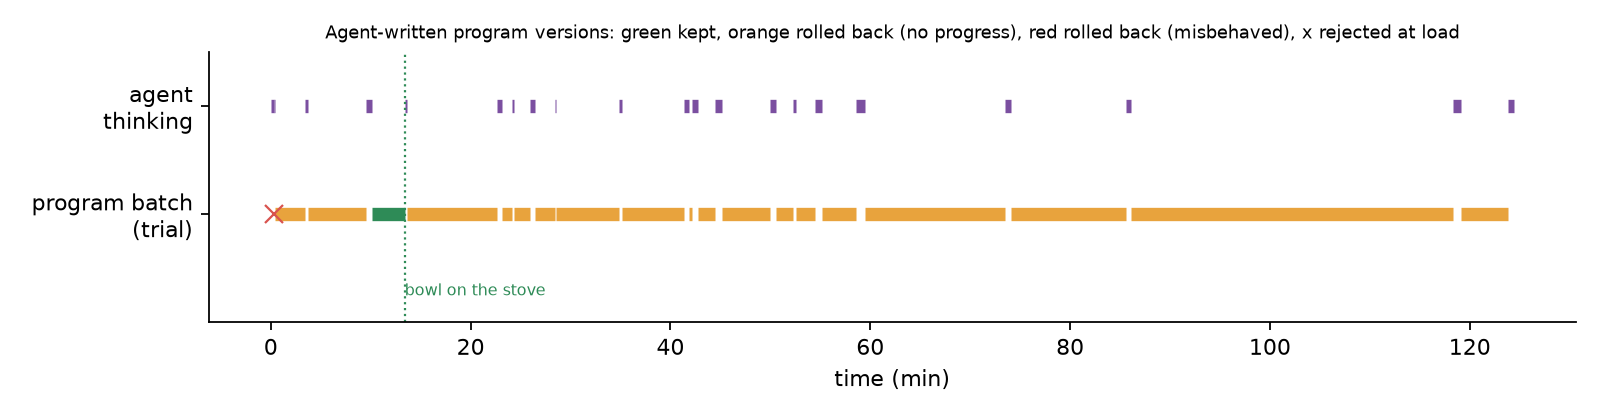
\includegraphics[width=\textwidth]{fig_libero_run2.png}
\caption{The 150-minute run: agent replies (top) and program batches on trial (bottom; green kept, orange rolled back, x rejected at load). Dotted line: the bowl reaches the stove.}
\end{figure}

\textbf{What this shows and does not.} It shows the loop running unattended for hours with a real VLA on the same computer: an agent writing, testing and replacing its own skills live, with bad versions rolled back and control timing unaffected. It does not show task success: with an off-the-shelf VLA and no task-specific training, the agent completed one of three goal facts. Logs, prompts, reasoning, plugins and videos are included with the code.

\section*{S12. Limitations}
Simplified simulations (kinematic, MuJoCo SO-101 and LIBERO), a stand-in VLA (the real SmolVLA only in S3, S9 and S11) and small planted bugs validate runtime mechanisms, not task reliability or agent capability. Both machines are virtual machines with two vCPUs; A shows occasional stall bursts even with Rust alone. Plugins run in the same Python process and could bypass the runtime (e.g., write shared memory directly); effects without a declared undo are detected, not reverted; the watchdog cannot interrupt a call blocked inside C code.

\medskip
\textbf{Code.} Rust loop, Python runtime, plugins, faulty repairs, agent harness (prompts included) and experiment scripts are included with this supplement.
\end{document}
